\chapter{Experiment}
\label{chap:experiment}


\section{Case Study: JGAP}
\label{sec:experiment_case_study}
\begin{table}[!b]
  \centering
  \rowcolors{2}{gray!30}{gray!20}
  \begin{tabular}{|l|r|r|}
    \hline
    \rowcolor[RGB]{169,196,223}
    \textbf{JGAP Source Artifacts} & \textbf{\# in Source} & \textbf{\# in Test} \\
    \hline Classes & 415 & 180 \\
    \hline Methods & 3017 & 1626 \\
    \hline LOC & 28975 & 19556 \\
    \hline JUnit Test Cases & -- & 1412\footnotemark[1] \\
    \hline
  \end{tabular}
  \caption{The amount of classes, methods, lines of code (LOC), and JUnit test cases in the JGAP repository}
  \label{tab:jgap_source_stats}
\end{table}

A preliminary evaluation of our mutation score predictor was preformed on JGAP (version 3.6.1), an open source genetic algorithm and genetic programming framework for Java, which was selected due to its comprehensive and mature JUnit test suite~\cite{JGAP}. Basic source code metrics for JGAP are provided in Table~\ref{tab:jgap_source_stats}. JGAP contains 1387\footnote{JGAP has 1412 JUnit test cases in total, however 25 of the tests caused errors in the Javalanche tool and were removed.} usable JUnit test cases. For JGAP, Javalanche generated 32031 mutants using the method-level mutation operators (see Section~\ref{subsec:background_javalanche}) of which only 18378 were actually covered by JGAP's test suite. We only considered the set of covered mutations in our approach as the mutations not covered contained no associated test cases. Considering only the covered mutants, JGAP's test suite killed 13698 mutants in 688 minutes and 43 seconds\footnote{Results from Javalanche on Intel Core i7-870 processor @ 2.93 GHz (with no parallel task execution).} resulting in an overall mutation score of 74.53\%.


\section{Results}
\label{sec:experiment_results}
We gathered 695 method-level data points and 127 class-level data points from JGAP. We first decided to view the distribution of JGAP's mutation scores (see Figure~\ref{fig:mutation_distributions_class}~\&~\ref{fig:mutation_distributions_method}). It is clearly obvious that the distribution for both classes and methods are more heavily dense for high mutation scores. As discussed in Section~\ref{sec:approach_training} we categorize the collected data into three groups of \textit{low, medium, high} mutation scores. Ideally we would have liked to have sufficient data coverage, such that we can use simple categories such as 0\%--33\% (\textit{low}), 33\%-66\% (\textit{medium)} and 66\%-100\% (\textit{high}). Based on the distribution of mutation scores in JGAP we instead decided to categorize our data such that one third of our data fall into each category (see Table~\ref{tab:results_details}).

\begin{figure}[!t]
  \centering
  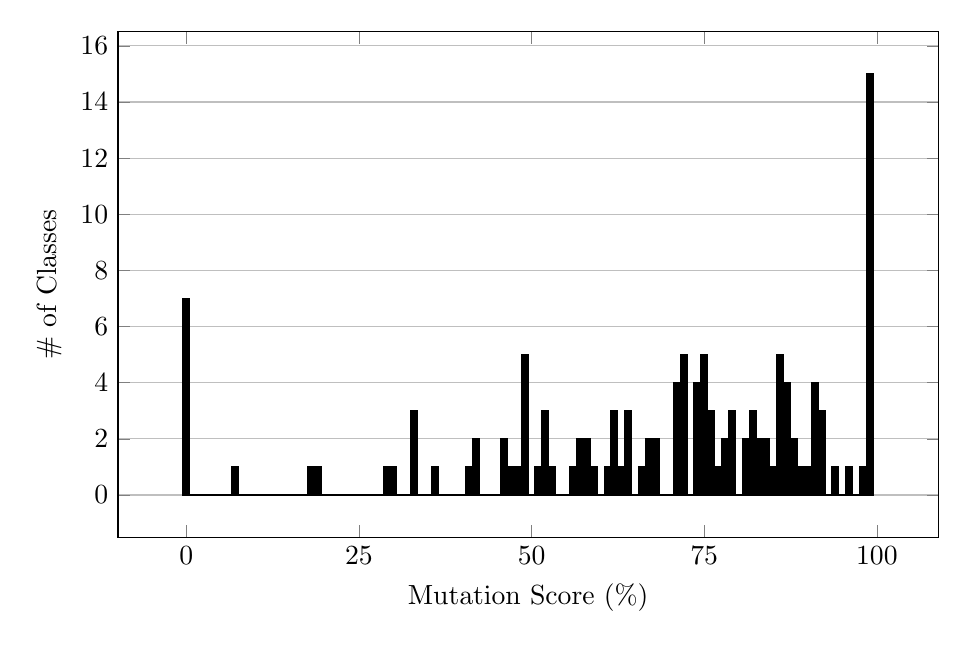
\begin{tikzpicture}
  \begin{axis}[
      xtick={0, 25, 50, 75, 100},
      ytick={0, 2, 4, 6, 8, 10, 12, 14, 16},
      bar width=1,
      ymajorgrids=true,
      xlabel=Mutation Score (\%),
      ylabel=\# of Classes,
      width=12.0cm,
      height=8.0cm]
      \addplot[ybar,fill=black] coordinates {
(0, 7) (1, 0) (2, 0) (3, 0) (4, 0) (5, 0) (6, 0) (7, 1) (8, 0) (9, 0) (10, 0) (11, 0) (12, 0) (13, 0) (14, 0) (15, 0) (16, 0) (17, 0) (18, 1) (19, 1) (20, 0) (21, 0) (22, 0) (23, 0) (24, 0) (25, 0) (26, 0) (27, 0) (28, 0) (29, 1) (30, 1) (31, 0) (32, 0) (33, 3) (34, 0) (35, 0) (36, 1) (37, 0) (38, 0) (39, 0) (40, 0) (41, 1) (42, 2) (43, 0) (44, 0) (45, 0) (46, 2) (47, 1) (48, 1) (49, 5) (50, 0) (51, 1) (52, 3) (53, 1) (54, 0) (55, 0) (56, 1) (57, 2) (58, 2) (59, 1) (60, 0) (61, 1) (62, 3) (63, 1) (64, 3) (65, 0) (66, 1) (67, 2) (68, 2) (69, 0) (70, 0) (71, 4) (72, 5) (73, 0) (74, 4) (75, 5) (76, 3) (77, 1) (78, 2) (79, 3) (80, 0) (81, 2) (82, 3) (83, 2) (84, 2) (85, 1) (86, 5) (87, 4) (88, 2) (89, 1) (90, 1) (91, 4) (92, 3) (93, 0) (94, 1) (95, 0) (96, 1) (97, 0) (98, 1) (99, 15)
      };
  \end{axis}
  \end{tikzpicture}
  \caption{The mutation score distribution of JGAP's classes that can be used for training.}
  \label{fig:mutation_distributions_class}
\end{figure}

\begin{figure}[!t]
  \centering
  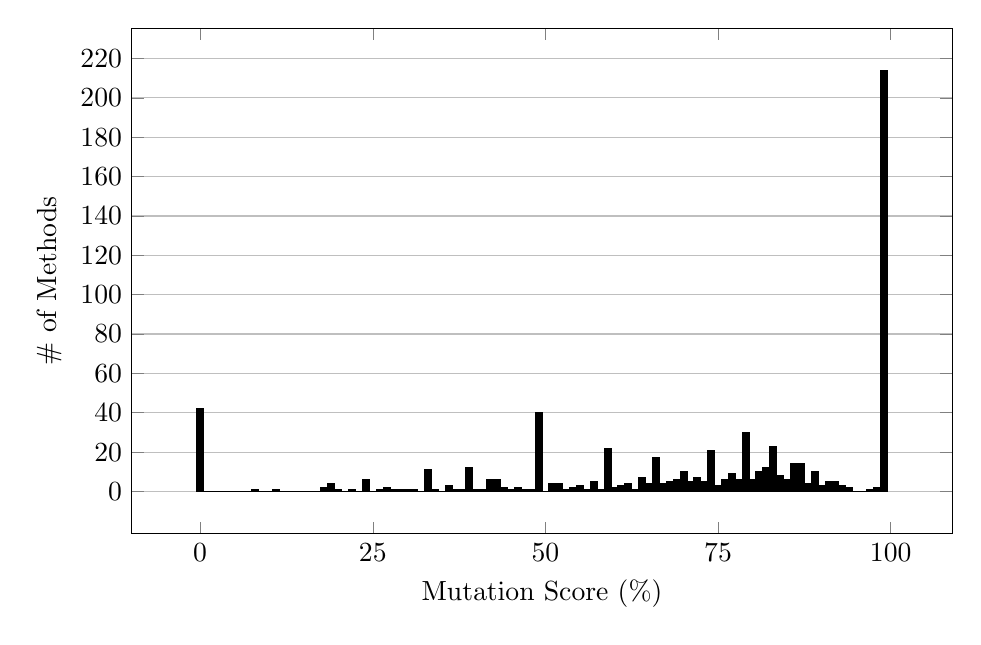
\begin{tikzpicture}
  \begin{axis}[
      xtick={0, 25, 50, 75, 100},
      ytick={0, 20, 40, 60, 80, 100, 120, 140, 160, 180, 200, 220},
      bar width=1,
      ymajorgrids=true,
      xlabel=Mutation Score (\%),
      ylabel=\# of Methods,
      width=12.0cm,
      height=8.0cm]
      \addplot[ybar,fill=black] coordinates {
(0, 42) (1, 0) (2, 0) (3, 0) (4, 0) (5, 0) (6, 0) (7, 0) (8, 1) (9, 0) (10, 0) (11, 1) (12, 0) (13, 0) (14, 0) (15, 0) (16, 0) (17, 0) (18, 2) (19, 4) (20, 1) (21, 0) (22, 1) (23, 0) (24, 6) (25, 0) (26, 1) (27, 2) (28, 1) (29, 1) (30, 1) (31, 1) (32, 0) (33, 11) (34, 1) (35, 0) (36, 3) (37, 1) (38, 1) (39, 12) (40, 1) (41, 1) (42, 6) (43, 6) (44, 2) (45, 1) (46, 2) (47, 1) (48, 1) (49, 40) (50, 0) (51, 4) (52, 4) (53, 1) (54, 2) (55, 3) (56, 1) (57, 5) (58, 1) (59, 22) (60, 2) (61, 3) (62, 4) (63, 1) (64, 7) (65, 4) (66, 17) (67, 4) (68, 5) (69, 6) (70, 10) (71, 5) (72, 7) (73, 5) (74, 21) (75, 3) (76, 6) (77, 9) (78, 6) (79, 30) (80, 6) (81, 10) (82, 12) (83, 23) (84, 8) (85, 6) (86, 14) (87, 14) (88, 4) (89, 10) (90, 3) (91, 5) (92, 5) (93, 3) (94, 2) (95, 0) (96, 0) (97, 1) (98, 2) (99, 214)
      };
  \end{axis}
  \end{tikzpicture}
  \caption{The mutation score distribution of JGAP's methods that can be used for training.}
  \label{fig:mutation_distributions_method}
\end{figure}

\begin{table}[!b]
  \centering
  \rowcolors{2}{gray!30}{gray!20}
  \begin{tabular}{|l|r|r|}
    \hline
    \rowcolor[RGB]{169,196,223}
    \textbf{Category} & \textbf{Class Mutation Score} & \textbf{Method Mutation Score} \\
    \hline low & 0.00\% -- 62.75\% & 0.00\% -- 66.66\% \\
    \hline medium & 62.75\% -- 83.25\% & 66.66\% -- 90.90\% \\
    \hline high & 83.25\% -- 100.00\% & 90.90\% -- 100.00\% \\
    \hline
  \end{tabular}
  \caption{The mutation score ranges that equally partition the datasets into three mutation score categories.}
  \label{tab:results_details}
\end{table}

Due to the small amount of data acquired from this experiment we decided to evaluate our results by performing a 10-fold cross-validation of our datasets. Our achieved cross-validation accuracy of JGAP (with all features from Table~\ref{tab:metrics}) was 58.27\% for class mutation scores and 54.82\% for method mutation scores. Figure~\ref{fig:confusion_matrix} illustrates a confusion matrix of the predicted values created from the SVM data for our three categories. It is also worth mentioning that our achieved accuracy outperforms random (which has an accuracy of 33.33\% given our category distributions) by 24.94\% for classes and 21.49\% for methods.

\begin{figure}[!t]
  \centering
  \begin{tikzpicture}[
  box/.style={draw,rectangle,minimum size=1.0cm,text width=2.0cm,align=center}]
    \matrix (confusion_matrix) {
      \node (actual_low_prediction_low)
      [box,
        label=left:$\mathbf{L'}$,
        label=above:$\mathbf{L}$
      ] {29, 108};
      &
      \node (actual_low_prediction_medium)
      [box,
        label=above:$\mathbf{M}$
      ] {7, 54};
      &
      \node (actual_low_prediction_high)
      [box,
        label=above:$\mathbf{H}$
      ] {7, 74};
      \\
      \node (actual_medium_prediction_low)
      [box,
        label=left:$\mathbf{M'}$
      ] {11, 43};
      &
      \node (actual_medium_prediction_medium)
      [box] {20, 112};
      &
      \node (actual_medium_prediction_high)
      [box] {11, 72};
      \\
      \node (actual_high_prediction_low)
      [box,
        label=left:$\mathbf{H'}$
      ] {8, 31};
      &
      \node (actual_high_prediction_medium)
      [box] {9, 40};
      &
      \node (actual_high_prediction_high)
      [box] {25, 161};
      \\
    };
    \node [left=-.1cm of confusion_matrix,text width=1.5cm,align=right] {\textbf{Actual \\ Value}};
    \node [above=-.1cm of confusion_matrix] {\textbf{Prediction Value}};
  \end{tikzpicture}
  \caption{Confusion matrix of mutation score prediction for JGAP.}
  \vspace{1mm}
  \footnotesize{\emph{Figure~\ref{fig:confusion_matrix} shows the confusion matrixs of (class, method) mutation score prediction for JGAP using all feature sets from Table~\ref{tab:metrics}. The first value in each cell represents the class value while the second represents the method value. $\mathbf{L}$ = Low, $\mathbf{M}$ = Medium and $\mathbf{H}$ = High.}}
  \vspace{1mm}
  \label{fig:confusion_matrix}
\end{figure}

We also conducted the cross-validation using subsets of our feature set and found that the combination of both source code and test suite features slightly improves the prediction accuracy (see Table~\ref{tab:subset_accuracy}).

\begin{table}[!t]
  \centering
  \rowcolors{2}{gray!30}{gray!20}
  \begin{tabular}{|c|r|r|}
    \hline
    \rowcolor[RGB]{169,196,223}
    \textbf{Set} & \textbf{Class Accuracy} & \textbf{Method Accuracy} \\
    \hline \ding{172} & 53.54\% & 48.77\% \\
    \hline \ding{173} & 49.61\% & 47.63\% \\
    \hline \ding{174} & 45.67\% & 49.78\% \\
    \hline \ding{175} & 54.33\% & 33.96\% \\
    \hline\ \textbf{\ding{172} \ding{173} \ding{174} \ding{175}} & \textbf{58.27\%} & \textbf{54.82\%} \\
    \hline
  \end{tabular}
  \caption{The cross validation accuracy of each feature subset for JGAP.}
  \vspace{1mm}
  \footnotesize{\emph{Table~\ref{tab:subset_accuracy} shows the cross validation (10-folds) accuracy of each feature subset (see Table~\ref{tab:metrics}) and all the four feature subsets combined for JGAP.}}
  \vspace{1mm}
  \label{tab:subset_accuracy}
\end{table}


\section{Experimental Setup}
\label{sec:experiment_setup}


\section{Experimental Subjects}
\label{sec:experiment_subjects}


\section{Experimental Results}
\label{sec:experiment_results}
